%  LaTeX support: latex@mdpi.com 
%  In case you need support, please attach all files that are necessary for compiling as well as the log file, and specify the details of your LaTeX setup (which operating system and LaTeX version / tools you are using).

%=================================================================
\documentclass[ijgi,article,submit,moreauthors,pdftex]{Definitions/mdpi} 

\usepackage{graphicx}
\usepackage{wrapfig}
\usepackage{lscape}
\usepackage{rotating}
\usepackage{epstopdf}
\usepackage{svg}
\usepackage{tabularx}


\newcommand{\specialcell}[2][c]{%
  \begin{tabular}[#1]{@{}c@{}}#2\end{tabular}}
%=================================================================
\firstpage{1} 
\makeatletter 
\setcounter{page}{\@firstpage} 
\makeatother
\pubvolume{xx}
\issuenum{1}
\articlenumber{5}
\pubyear{2019}
\copyrightyear{2019}
%\externaleditor{Academic Editor: name}
\history{Received: date; Accepted: date; Published: date}
%\updates{yes} % If there is an update available, un-comment this line

%% MDPI internal command: uncomment if new journal that already uses continuous page numbers 
%\continuouspages{yes}

%------------------------------------------------------------------
% The following line should be uncommented if the LaTeX file is uploaded to arXiv.org
%\pdfoutput=1

%=================================================================
% Add packages and commands here. The following packages are loaded in our class file: fontenc, calc, indentfirst, fancyhdr, graphicx, lastpage, ifthen, lineno, float, amsmath, setspace, enumitem, mathpazo, booktabs, titlesec, etoolbox, amsthm, hyphenat, natbib, hyperref, footmisc, geometry, caption, url, mdframed, tabto, soul, multirow, microtype, tikz

%=================================================================
%% Please use the following mathematics environments: Theorem, Lemma, Corollary, Proposition, Characterization, Property, Problem, Example, ExamplesandDefinitions, Hypothesis, Remark, Definition, Notation, Assumption
%% For proofs, please use the proof environment (the amsthm package is loaded by the MDPI class).

%=================================================================
% Full title of the paper (Capitalized)
%\Title{Using dockers for reproducible science in the geospatial domain}
%\Title{Evaluating and Enhancing Open Reproducible Research in GIScience using Containerisation Solutions}
%[Result]: A [method] study of [topic] among [sample]
\Title{Leveraging container technologies in a GIScience project: a perspective from Open Reproducible Research}

% Author Orchid ID: enter ID or remove command
\newcommand{\orcidauthorA}{0000-0003-2501-484X} % Add \orcidA{} behind the author's name
\newcommand{\orcidauthorB}{0000-0002-9304-0719} % Add \orcidB{} behind the author's name
\newcommand{\orcidauthorC}{0000-0002-8718-218X} % Add \orcidC{} behind the author's name

% Authors, for the paper (add full first names)
\Author{Benito M. Zaragozí$^{1,\dagger}$\orcidA{}, Sergio Trilles$^{2,\dagger}$*\orcidB{}, José T. Navarro-Carrión$^{3}$\orcidC{}}

% Affiliations / Addresses (Add [1] after \address if there is only one affiliation.)
\address{%
$^{1}$ Departament de Geografia, Universitat Rovira i Virgili, C/ Joanot Martorell, 43480, Vilaseca, Spain\\
$^{2}$ Institute of New Imaging Technologies (INIT), Universitat Jaume I, Av. Vicente Sos Baynat s/n, 12071, Castell\'o de la Plana, Spain\\
$^{3}$ Instituto Interuniversitario de Geograf\'ia (IIG), Universidad de Alicante, C/ San Vicente s/n, 03690, Alicante, Spain\\}

% Contact information of the corresponding author
\secondnote{The authors contributed equally to this work.}
\corres{strilles@uji.es, Tel. (+34) 964 38 76 86.}
% Author Orchid ID: enter ID or remove command

\abstract{Scientific reproducibility is essential for the advancement of science. It allows the results of previous studies to be reproduced, validates their conclusions and develops new contributions based on previous research. Nowadays, more and more authors consider that the ultimate product of academic research is the scientific manuscript, together with all the necessary elements (i.e. code and data) so that others can reproduce the results. However, there are numerous difficulties for some studies to be reproduced easily (i.e. biased results, the pressure to publish or proprietary data, among others). 
In this context, we explain our experience in an attempt to improve the reproducibility of a GIScience project. According to our project needs, we evaluated a list of practices, standards and tools that may facilitate open and reproducible research in the geospatial domain, contextualising them on Peng's reproducibility spectrum. Among these resources, we focused on containerisation technologies and performed a shallow review to reflect on the level of adoption of these technologies in combination with OSGeo software. Finally, containerisation technologies proved to enhance the reproducibility, and we used UML diagrams to describe representative work-flows deployed in our GIScience project.} 

% Keywords
\keyword{reproducibility; open science; open reproducible research; GIScience; containerisation; dockers; UML}

% The fields PACS, MSC, and JEL may be left empty or commented out if not applicable
%\PACS{J0101}
%\MSC{}
%\JEL{}

%%%%%%%%%%%%%%%%%%%%%%%%%%%%%%%%%%%%%%%%%%
%\setcounter{secnumdepth}{4}
%%%%%%%%%%%%%%%%%%%%%%%%%%%%%%%%%%%%%%%%%%

\begin{document}

%%%%%%%%%%%%%%%%%%%%%%%%%%%%%%%%%%%%%%%%%%
\section{Introduction}
\label{sec:introduction}

Replicability and reproducibility are essential aspects of the scientific method that add consistency to scientific contributions in any discipline. The reproduction of any scientific work seeks to verify and validate the results obtained, which will lead to a better understanding of the realm that has been studied. This approach increases the chances of reusing or extending previous research works \citep{Meng2015a}.

The statement ``Replicability is not reproducibility'' has already been discussed in various works. In \cite{barba2018terminologies}, the author distinguishes between reproducibility and replicability, arguing that replication is a study that arrives at the same scientific findings as another study, collecting new data and completing new analyses. As far as research can provide all the necessary data and the computer codes to rerun the analysis to re-create the results, it can be considered reproducible research. In other words, reproducibility refers to a phenomenon that can be predicted to be repeated under the same experimental conditions. At the same time, replicability describes the ability to obtain an identical result when an experiment is performed under new conditions (data and methods). This distinction makes more sense in the computer sciences field, more specifically in computational research, because if data and code are available, the results should be identical. It must be taken into account that replicability does not guarantee the validity of the scientific contribution \citep{peng2011reproducible}.

A full degree of reproducibility or replicability will not always be possible, as it dramatically increases the cost of studies and the researchers' workload \citep{stodden2012reproducible}. This statement is also becoming increasingly evident in studies related to computer science. In the last two decades, a vast amount of data has been collected and will continue to grow exponentially. The term ``Big Data'' refers to an enormous volume of data that exceeds the capabilities of conventional database systems because the data is too bulky, recorded too fast or is not structured according to the existing database architectures \citep{Brunsdon2014a}. The phenomenon of Big Data makes it challenging to reproduce certain studies -- usually for reasons related to time, resources and labour -- and so only a well-founded suspicion about the results would make it necessary to repeat the computational experiences \citep{Gil2016a}.

Over the last decade, the concern to determine to what extent studies published in scientific journals are reproducible has been widely discussed. Some data can be alarming and, in other studies, authors can talk of a ``reproducibility crisis'' \cite{Begley2015a, Baker2016}, to the point that 90\% of participants in a recent survey of the journal Nature agreed that the aforementioned crisis exists \cite{Baker2016}. Some more striking figures estimate that 85\% of biomedical research efforts are wasted \cite{Begley2015a}, while \cite{Freedman2015a} have calculated that -- only in the USA -- 28,000 million dollars are spent every year on research that is not reproducible.

The risks of the lack of reproducibility are also manifested in the social sciences. An example of this is the article by Reinhart and Rogoff in 2010 \citep{Reinhart2010a}, which was published in a special issue (without peer review) of the prestigious journal \textit{The American Economic Review}. Its results were taken as essential arguments to support pro-austerity policies applied after the economic crisis that began in 2007--2008. Later, it was shown that the results could not be reproduced due to errors in the coding of the data of a spreadsheet, selective exclusion of available data and a low weighting of variables. As a result, the phenomenon studied would be much less significant than the authors of the first article indicated \citep{Herndon2014a,Reinhart2010a}. If political decisions are to be based on scientific studies from the social sciences, it is logical to expect such studies to be fully reproducible \cite{Brunsdon2014a}.

Although some authors use the term ``crisis'' to describe the widespread lack of reproducibility, it must be remembered that science is a cumulative process and that many studies are needed to generate new knowledge. To a greater or lesser extent, the lack of reproducibility is part of the essential functioning of science, which continuously corrects itself \cite{OpenScienceCollaboration2015a}. In any case, there is much room for the improvement of research practices and thus being able to make better use of the resources allocated for science.

Researchers from different disciplines have begun to promote reproducible research as a minimum standard to defend the results of research, especially in studies in which obtaining complete replicability is not viable \cite{Peng2011a}. In this way, reproducibility is defined as a spectrum of possibilities between an investigation that cannot be validated and another that is fully replicable (see Figure \ref{fig:reproducibility_spectrum}).

\begin{figure}[!ht]
  \centering
  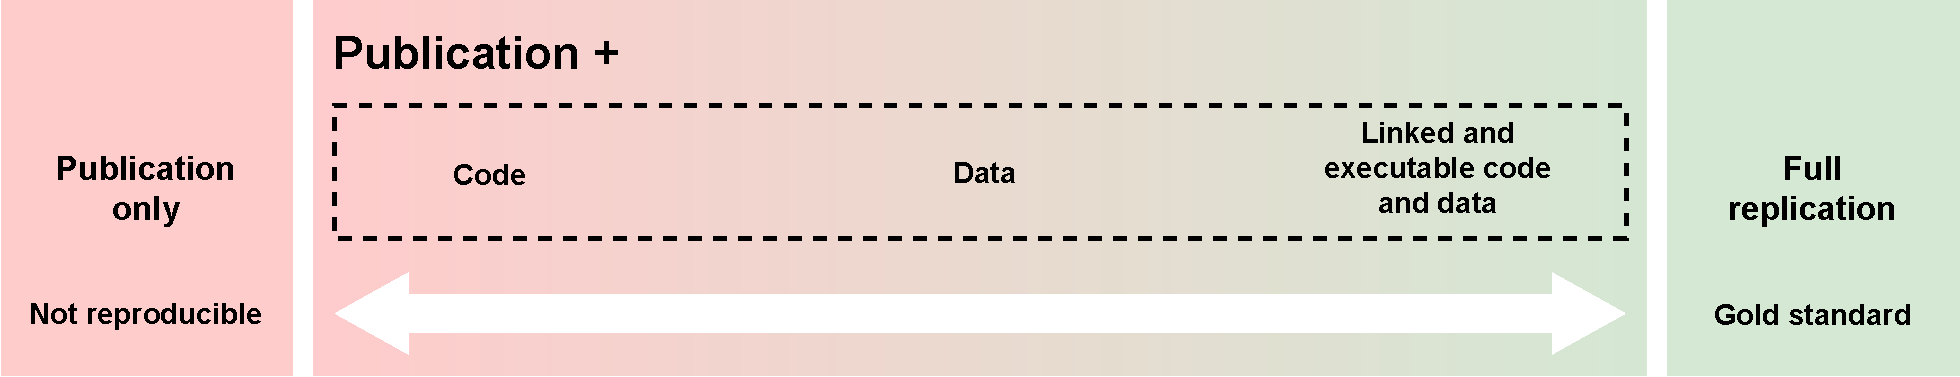
\includegraphics[width=\textwidth]{images/fig1.pdf}
  \caption{The spectrum of scientific reproducibility, between a scientific publication and full replication (based on \cite{Peng2011a}).}
  \label{fig:reproducibility_spectrum}
\end{figure}

Obviously, to achieve a high degree of reproducibility, it is necessary to maintain detailed documentation and to describe the methods applied meticulously. Traditionally, scientific publications have been used for this purpose. However, as certain studies increase in complexity, it becomes clear that just papers -- text, tables and static figures -- are no longer enough to reproduce a scientific study \cite{Stodden2014}. Researchers should include textual and numerical descriptions of the research, as well as other essential elements, such as software, data, environment variables, platform dependencies and other resources involved in the methodology used \cite{Singleton2016b}.

This research work focuses on reproducibility in the field of Geographic Information Science \cite{goodchild1992geographical} (also GIScience or GISc), which comprises a wide range of research areas, such as climate modelling \cite{Peng2011a} or studies on the applicability of Voluntary Geographic Information (VGI) \cite{Ostermann2017a}, among others. Besides, special attention is also paid to the Open Reproducible Research (ORR) perspective, which is exemplified as a research work where all the elements (i.e. data, code, etc.) are based on open and publicly accessible resources that can produce the same results as those that have been published \cite{goodman2016does}. The concept of reproducibility is addressed here in a broader sense, including works with different levels of configuration and development needs (e.g. from geostatistical experiments to new software development). It is considered that something cannot be understood as being reproducible without it being open \cite{pontika2015fostering}. In this sense, ORR must be Open Science (OS) and should meet the following requirements: 1) open access, which refers to the possibility of accessing research results (publications) for free, without restrictions \cite{antelman2006open}; 2) open data, which is based on the publication of research data collected during the research process and made available to the community for study and reuse \cite{murray2008open} using a license; and 3) open-source, which refers to software whose source code is publicly available along with a licence that allows its use, modification and distribution \cite{perens1999open}.


\subsection{The SIOSE-INNOVA project}
\label{subsec:siose}

As just explained, the concern for scientific reproducibility is present in many researchers and is taken into account in more and more projects. Accordingly, in 2017, when we started the SIOSE-INNOVA project, we evaluated how we would ensure that our project did not suffer from the problems mentioned in the previous section. To understand the rest of this work and our decisions, in this subsection we introduce the main details and requirements of the project.

The Information System on Land Occupation of Spain (SIOSE; \url{https://www.siose.es/}) mainly involves managing the creation and maintenance of a geodatabase that contains land occupation data (land use/land cover; LU/LC) from Spain. This data is necessary for researchers studying different environmental and socioeconomic problems. The SIOSE geodatabase contains a big volume of vector LU/LC data at a 1:25,000 scale, comprising about 10 GB in each of the published database versions (2005, 2009, 2014 and 2019). These volumes are going to be much more important in the future high-resolution versions that will reach the cadastral parcel scale. This database follows a complex (object-oriented) database model that is cumbersome for typical GIScience projects. These limitations are closely related to the previously commented reproducibility problems. As explained before, working with such big databases and complex data models makes reproducing any workflow much more difficult unless proper practices are applied.

The SIOSE-INNOVA project (\url{http://siose-innova.es/}) proposes technical and methodological innovations for the SIOSE database. These innovations are considered necessary to make this data more accessible for its application in geographical studies. The SIOSE-INNOVA project is organised in two complementary parts: 1) a technical innovation part that consists in verifying which open source technologies provide the best solutions to exploit certain facets of the SIOSE database, and 2) an applied part that involves the implementation of these new technologies in real case studies. In this project, experts with very different technological profiles -- GIS, geodatabases, programming, data mining, among other tools -- need to collaborate and overcome the difficulties in using the SIOSE database. All these specialists must be able to work with the same tools, and the only possibility is that some intermediary provides a stable and transparent working environment.

SIOSE data are public and distributed under a CC-BY 4.0 licence. This licence allows free access and free use for any legitimate purpose, the only strict obligation being to acknowledge and mention the origin and ownership of licensed geographic information products and services, such as the Instituto Geográfico Nacional (IGN). SIOSE data can be retrieved from the downloads page of the Centro Nacional de Información Geográfica (CNIG) \cite{cnig} or the websites of Spanish regional mapping agencies.

As mentioned above, the SIOSE database is designed according to an object-oriented model, but due to practical reasons it is adopted and implemented within an object-relational database, which is a clear example of the \textit{object-relational impedance mismatch} \cite{NavarroCarrion2016}. The usability problem investigated by the SIOSE-INNOVA project has to deal with the fact that regular users of this type of information layers usually work with \textit{ESRI Shapefiles} and these are generally not used to work with such information in any of the original distributions of SIOSE (corporate databases). These problems could be solved with the development of new tools for querying the database, which implies the need to define a working environment in which the development becomes manageable, and everyone involved can collaborate in the realisation of computational experiments. This could be understood as ``intra-project reproducibility'', but that would have positive effects on higher reproducibility and sustainability also by researchers not belonging to this project.

\subsection{Objectives}
\label{subsec:objectives}

The requirements of the SIOSE-INNOVA project led us to investigate how GIScientists use open source tools and techniques to produce ORR outcomes. Only then would it be possible to make good use of those resources in specific GISc projects. In this manuscript, we explain this process of discovery by providing some context information and describing how we finally addressed reproducibility in our project.

The target audience of this work is researchers and practitioners -- with or without much experience in ORR -- who wish to explore how to produce reproducible research in the GIScience domain. Considering this audience and the SIOSE-INNOVA requirements, the specific objectives of this work are: 1) to define the most essential facilitating technologies, platforms and good practices that enhance ORR; 2) to provide an overview on how containerisation technologies can boost reproducibility in GIScience projects; 3) to analyse the level of adoption of containerisation technologies in the geospatial domain; and 4) to describe the challenges that must be overcome to integrate reproducible workflows into GISc projects with requirements similar to those of the SIOSE-INNOVA project.

The rest of the paper is organised as follows. Section \ref{sec:GISreproducibility} presents how ORR can be achieved within the scope of GIScience. Section \ref{sec:dockerhub} shows the impact of reproducibility on GIScience using the \textit{Docker Hub} repository as a proxy. Section \ref{sec:projects} describes how ORR was achieved in different computational experiences involving a SIOSE database. The paper finishes with Section \ref{sec:conclusions}, which presents the conclusions and proposes lines for future work.

%----------------------------------------------------------

\section{Open Reproducible Research in the geospatial domain}
\label{sec:GISreproducibility}

GIScience shares the concerns as mentioned above about reproducibility. However, on analysing the literature published in the field of geospatial sciences, it can be observed that their presence is much lower than in other disciplines \cite{giraud2017reproducible}. 

Due to the importance of this topic, several studies assess the application of ORR in GISc. For example, \cite{konkol2019computational} aims to analyse the reproducibility of the work of geoscientists who carry out computational research and to identify the obstacles hindering the achievement of reproducible works. In Ostermann and Granell \cite{ostermann2017advancing}, the authors researched reproducibility in VGI, where they obtained non-promising results as regards the degree of reproducibility. \cite{granell2018reproducible} proposed a short-term strategy to achieve reproducible research within the Association of Geographic Information Laboratories in Europe (AGILE) community \cite{agilewebsite}. In \cite{nust2018reproducible}, the same authors performed an analysis of 32 conference papers presented in the AGILE conferences, between 2010 and 2017, concluding that there is a low average level of reproducibility in GIScience and no positive trend is perceived. In \cite{skaggs2015reproducible}, the authors proposed a programme for submitting reproducible publications ---including data, source code and metadata--- in an open geosciences journal. \cite{nust2017opening} put forward the Executable Research Compendium (ERC), which uses \textit{Docker} containers to encapsulate in an environment with all components.

Many works in GISc build statistical models (computational research) from geospatial data. Of course, when they share their algorithms and data, they can be considered works that are reproducible without much difficulty \cite{konkol2019computational}. However, this type of work is not the most predominant in computationally intensive sciences, and on many occasions achieving reproducibility is not trivial. Most of the scientific work carried out in the computer science field requires complex environments -- with specific workflows -- for each of the problems to be investigated \cite{barga2010provenance}. Besides, geospatial datasets are not always easy to share, as they tend to be huge in terms of size or volume. As explained in Subsection \ref{subsec:siose}, this would be the case of the SIOSE-INNOVA project.

Nowadays, there are many available resources for addressing ORR, and we even knew many of these resources before starting the SIOSE-INNOVA project. In order to contextualise them, we propose a diagram based on the Peng's \cite{peng2011reproducible} reproducibility spectrum (see Figure \ref{fig:reproducibility_spectrum}). Our proposal is just a juxtaposition of the reproducibility spectrum proposed by Peng with a partially ordered space showing important \textit{practices}, \textit{platforms} and types of \textit{assets} that could be used in a GISc project. Although with certain precautions, we will refer to this diagram as the spectrum of reproducibility in GIScience (see Figure \ref{fig:GisReproSpectrum}). As in the original reproducibility spectrum, our proposal is divided into three main zones: 1) publication only (not reproducible in most cases); 2) publication with some elements that promote reproducibility (i.e. code, data, environments, \textit{assets}, \textit{platforms}, \textit{practices}, etc.); and 3) fully replication research. The elements required to ensure a good level of reproducibility will vary between projects and research objectives, so many combinations are possible. Of course, there is no universal solution that solves all cases. In this ORR spectrum, the key element is the level of commitment to achieve reproducibility. A higher level of commitment means developing all those elements that promote reproducibility in each particular case (i.e. \textit{assets}, \textit{platforms} and \textit{practices}).

\begin{figure}[!ht]
  \centering
  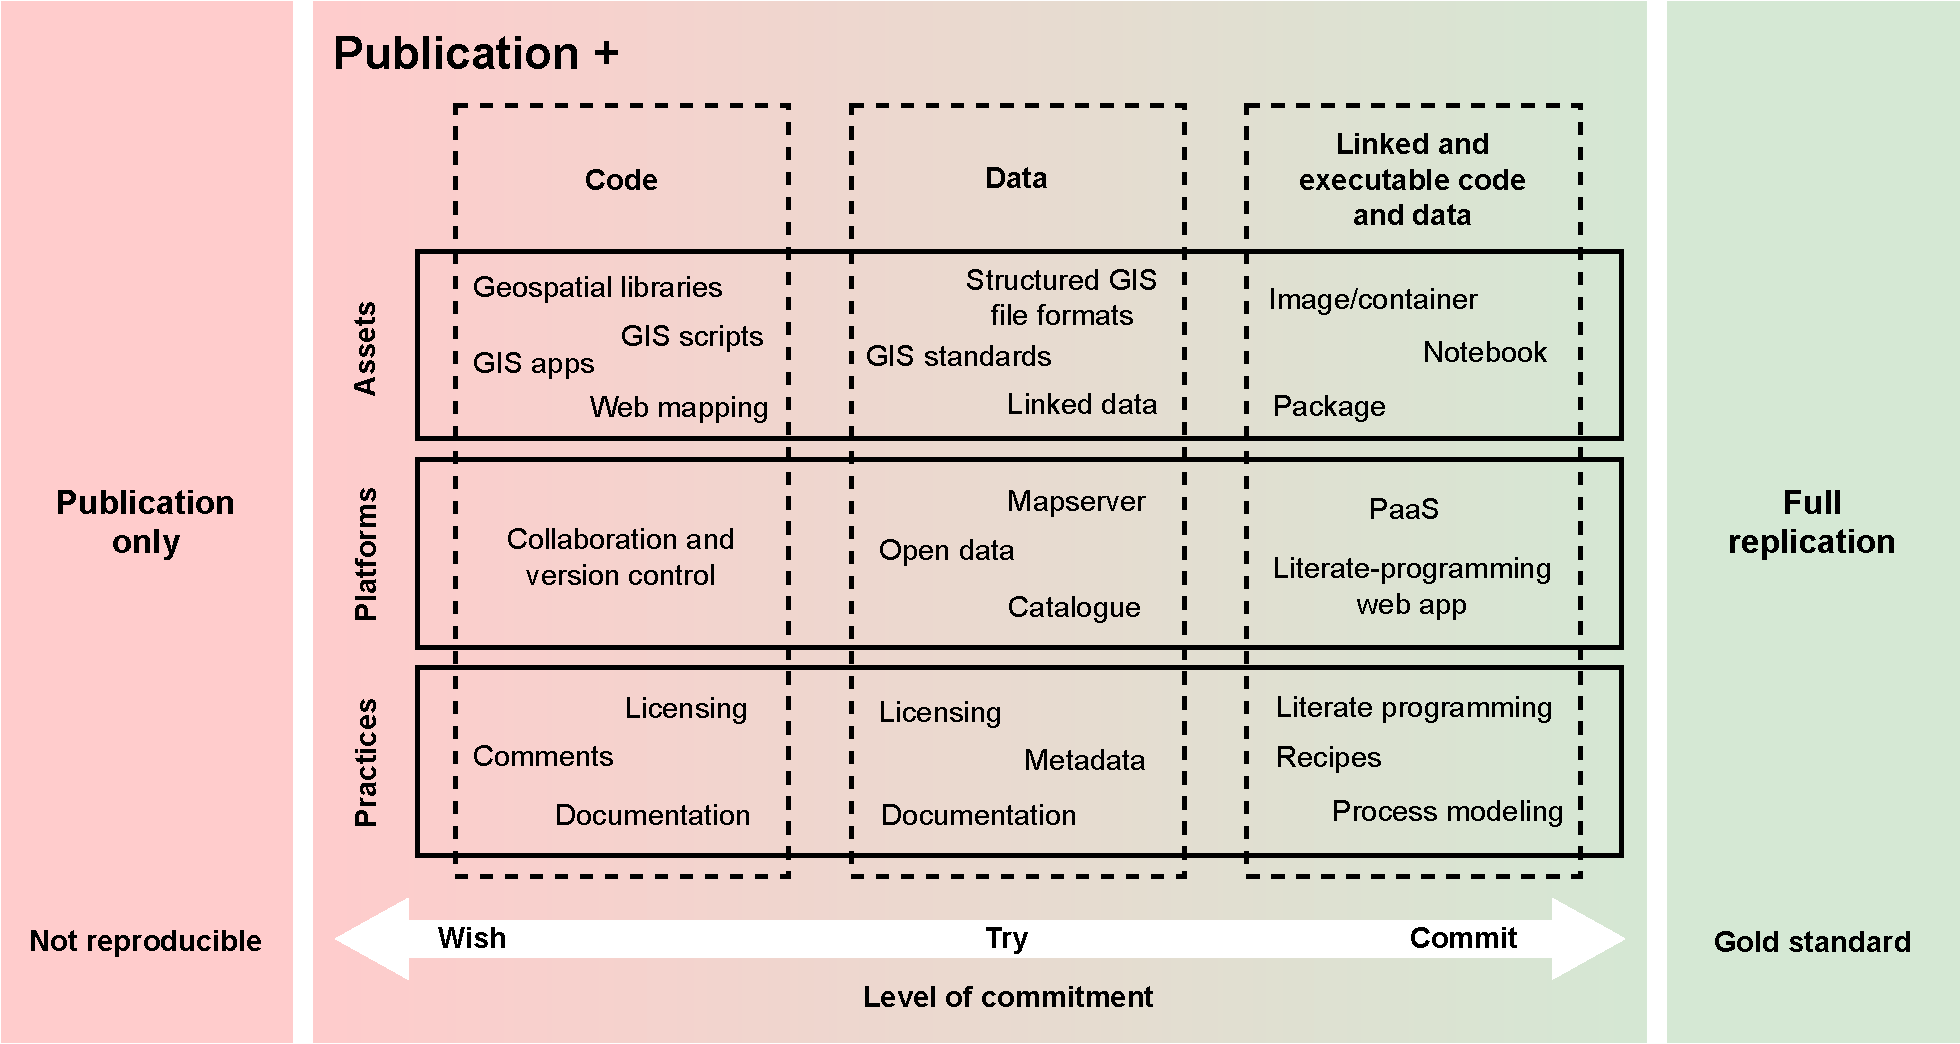
\includegraphics[width=\textwidth]{images/fig2.pdf}
  \caption{An Open Reproducible Research spectrum in the field of GISciences. Note: the relationships between the elements in the core of the diagram are not defined, so these will vary according to the needs of each project.}
  \label{fig:GisReproSpectrum}
\end{figure}

Another important particularity of this ORR spectrum is that many of the elements that promote reproducibility (e.g. \textit{assets}, \textit{platforms} or \textit{practices}) can accomplish very different purposes. For example, any of the development (collaboration and version control) \textit{platforms} -- \textit{GitHub}, \textit{Bitbucket} \cite{bitbucket} and \textit{Gitlab} \cite{gitlab} -- can be used for different functions in a reproducible project. They could be used for code sharing and versioning, project documentation and management, publishing small datasets, informing about the chosen licensing or even linking data and code in some web applications, among other possibilities. 

The inherent complexity of this spectrum means that in this work, we can only present a general context on specific \textit{practices} and tools that generally solve the most typical reproducibility problems. The following subsections detail how the reproducibility spectrum can be interpreted within the context of GIScience projects --- from the most elementary \textit{assets} (e.g. programming languages, data formats, etc) to their integration into the most common good \textit{practices} (those introduced in Figure \ref{fig:GisReproSpectrum}). In this work, we call \textit{assets} to the list of heterogeneous resources that may be used in the geospatial domain, such as programming libraries, desktop applications or implemented standards.


\subsection{Collaborative development and code sharing}
\label{subsec:code}

Reading the central zone of our spectrum -- from left to right and from top to bottom --, we first find what we have called code \textit{assets}, including free geospatial projects of different categories, such as programming libraries or desktop GIS applications, and products created for their usage. In the SIOSE-INNOVA project, this would be referred to spatial Data Base Management Systems (DBMS), database clients and scripts written in a database query language.

The decision of which tools are adequate for a particular GISc project depends on many factors, but it is essential to know the available options and their main characteristics. As a convention, geospatial projects can be grouped by software category or by programming language \cite{Steiniger2013, Steiniger2009}. Grouping projects by a programming language is interesting because it should be easier to use projects and reuse code developed with the same programming language. Depending on the particular objectives of a GISc project, many different programming languages can be used, but here we only focus on the most relevant ones. In decreasing order of usage \cite{index2018tiobe} the following are some of the most commonly used programming languages and projects under the Open Source Geospatial Foundation (OSGeo) \cite{osgeo} umbrella:

\begin{itemize}
\item \textit{Python}. This is the language with the greatest presence in the GIS realm. This is due to its use as a scripting language in the best-known GIS desktop applications, such as \textit{QGIS} \cite{qgis2015qgis}.
\item \textit{Javascript}. Widely used for web programming, it is the language with the most widespread presence in web mapping. Two well-known web mapping APIs are \textit{OpenLayers} \cite{hazzard2011openlayers} or \textit{Leaflet} \cite{leafletjs}.
\item \textit{R}. This language is used for statistical computing, data visualisation, data science and geospatial analysis. It can also be used to access other GIS or inside GIS tools such as \textit{QGIS} via connectors. The most relevant and useful R libraries are collected into the \textit{Spatial Task View} (\url{https://cran.r-project.org/view=Spatial}).
\item \textit{SQL}. For many years it has been used to query geospatial databases. \textit{SQL} is at the heart of many GIS operations in spatial queries. It is used in software such as \textit{PostGIS} \cite{postgis}, \textit{Spatialite} or \textit{QGIS}, among others.
\item \textit{Java}. This is one of the most widely used languages in open source GIS programs, such as \textit{GeoServer} \cite{geoserver}, \textit{GeoNetwork} \cite{geonetwork} or \textit{JTS} \cite{solutions2003jts}.
\item \textit{C/C++}. These languages are two of the most used for creating GIS desktop applications and other platforms. In the GIS field, we can find open source applications or libraries in this language, such as \textit{QGIS}, \textit{GRASS GIS} \cite{neteler2012grass}, \textit{MapServer} \cite{mapserver}, \textit{GDAL} \cite{gdal} or \textit{Orfeo Toolbox} \cite{orfeo}.
\end{itemize}

Among this list of programming languages and projects, the objectives of the SIOSE-INNOVA project can be better achieved using \textit{SQL} on a DBMS like \textit{PostgreSQL/PostGIS}. This solution can manage volumes of geospatial data similar to those in the SIOSE database without any problem. \textit{PostgreSQL} allows storing relational data or hierarchically structured data thanks to the \textit{JSONB} support, which is very convenient considering the object-oriented data model used by SIOSE.

Following with our spectrum of reproducibility, we consider the use of collaborative platforms for sharing code and keep it accessible at any version as essential. Code must be linked to research publications using permanent and stable public URIs. There are different collaboration and version control platforms that help to achieve these requirements (i.e. \textit{GitHub}, \textit{BitBucket} or \textit{GitLab}). These \textit{platforms} enable several people to work collaboratively on a single project and track all the contributions using unique identifiers for each contribution (e.g. git commit hashes or released versions). This last feature allows us to know exactly which version of the code was used to generate certain research results, which thus enables others to test modifications or to suggest improvements without affecting the normal development of the main project. Perhaps the essential feature of these development platforms is to generate a community that can continue development around the research questions \cite{ram2013git}. Even if the platforms mentioned above are not enough, there are more indicated solutions such as \textit{Archivematica} \cite{van2010archivematica} and \textit{RODA} \cite{faria2009roda} to preserve long-term access to trustworthy, authentic and reliable digital contents.

At the end of the first column of our spectrum, we locate the \textit{practices} that can contribute to sharing the code of GISc projects in the most appropriate way. Within the movement towards open science, the concept of open methods is defined \cite{whyte2011open}. This is based on the idea that researchers should document their methods as complete as possible \cite{nust2018reproducible}, including the provision of textual instructions or other material (photos, videos, etc.). Documenting the code, both at the level of general documentation and comments within the code itself, is a necessary practice to achieve reproducible research. Apart from the \textit{README} files that can describe each project in a general way, it is necessary to generate documentation that describes each component that has been developed.

Another critical aspect of the code to keep in mind is the type of licence attributed, which is also a notable metadata element. There is a general lack of knowledge about the meaning of each type of licence, which is one of the main barriers to reusing code (and data) \cite{benitez2018creating}. As far as we develop open research, open licences for reuse should be adopted, after evaluating the most appropriate choices \cite{stodden2008legal}.


\subsection{Geospatial data availability}
\label{sec:data}

Making a dataset accessible does not guarantee the reproducibility of research work but reduces the costs for reproducibility. For this reason, we are going to review the essential elements for publishing open geospatial data. In this subsection, we focus on the central part of our spectrum of reproducibility (Figure \ref{fig:GisReproSpectrum}).

In any discipline applied through computer science, there is a set of structured data formats used by its community. When these formats are widely known and based on open standards, they become a useful and interoperable means of sharing data. In the case of GIScience, there are mainly two essential data models with many file-types based on them: 1) vector files usually contain geometries defined by coordinate lists, which represent points, lines or polygons, and 2) raster files are bitmap images that can be used to store satellite images, elevation models, heat maps or other topographic representations. The most important file formats for both types are outlined below.

As mentioned in Subsection \ref{subsec:siose}, the SIOSE requirements for the data are the following: 1) to be stored in a vector format, 2) to hold a considerable volume of data -- that could be difficult to manage within specific data formats, and 3) to manage a hierarchical structure of land uses. The most appropriate data formats for a SIOSE database should fulfil these requirements. In this way, we present a selection of the vector data formats that are commonly used to publish data by the CNIG.

\begin{itemize}
\item \textit{ESRI Shapefile} \cite{esriShapefile}. This is a traditional and widely used vector data format. Normally, a \textit{Shapefile} encloses at least three or four different files (\textit{.shp}, \textit{.dbf}, \textit{.shx} and \textit{.prj}) and defines a single type of geometry, which implies that each \textit{Shapefile} can only store points, lines or polygons. This format, although widely used, was not intended as an open format when it was conceived. However, any GIScientist should know this format given the large amount of legacy data stored in this format and users that still use it.
\item \textit{GeoCSV} \cite{stults2015geocsv}. Comma-Separated Values (\textit{CSV}) is a vector file format  and is extensively used in any discipline. The \textit{CSV} format allows work to be carried out using the most usual programs, such as \textit{Excel} or \textit{Notepad}. \textit{CSV} is a plain text file where columns are separated using commas and rows by lines. More specifically, an optional geometry extension (\textit{GeoCSV}) has been created that can store points (latitude and longitude) and Well-Known Text (\textit{WKT}) standard geometries.
\item \textit{GeoJSON} \cite{butler2016geojson}. This is an extension of JavaScript Object Notation (\textit{JSON}) adding geospatial data. It offers the advantage of being a lightweight, easy-to-read notation for web applications. It is usually used as output for APIs and is a vector format.
\item \textit{Spatialite/SQLite} \cite{spatialite}. \textit{SpatiaLite} is an open source library that extends the \textit{SQLite} core with Spatial \textit{SQL} capabilities. This is conceptually similar to the combination of \textit{PostgreSQL/PostGIS}, but in this case \textit{Spatialite} is meant for embedded and portable geodatabases.
\item \textit{Geopackage} \cite{geopackage}. This format is a universal file format for sharing and transferring vector and raster spatial data. It is open and supported by Open Geospatial Consortium (OGC) \cite{ogc}. \textit{Geopackage} is backed by and extends \textit{SQLite} and is highly influenced by \textit{Spatialite}.
\item \textit{NetCDF} \cite{netCDF}. This is a data model for array-oriented scientific data that can also store both, vector and raster data. It is a recommended format to encode and distribute multi-dimensional and gridded geospatial data.
\end{itemize}

Before 2019, SIOSE databases were distributed in ESRI Shapefiles and other proprietary formats, but now data is internally managed using \textit{PostGIS} and can be downloaded as \textit{Geopackages} -- one for each of the 17 Spanish regions. As mentioned above, these solutions match the requirements and facilitate the introduction of new improvements, such as the storage of hierarchical data structures. Thus, these formats would also be the most adequate for the SIOSE-INNOVA project.

The choice of an appropriate data format is important for reproducibility to some degree but, any of the mentioned GIS formats come along with a variety of software libraries and tools that add more options to work with these data. Moreover, sharing GIS data files is not the only way to make data accessible. According to the \textit{5-star} open data classification (\url{http://5stardata.info/en/}) proposed by \cite{berners2006linked}, there are different levels of openness for sharing (GIS) data on the web. This scheme defines protocols and guidelines that endorse open data format and linkages among datasets, facilitating data interoperability within the context of a Web of Data \cite{bizer2009dbpedia}. In the GIScience community, the OGC standards have a goal to define an interoperable way to build data services on the web. These standards imply a considerable number of conventions (interfaces and encodings), but adhering to these standards guarantees interoperability \cite{percivall2010progress} and reuse, increasing the reproducibility of a work \cite{giuliani2019earth}. 

In the recent years, the OGC has performed an important task in order to publish different standards, proposing technical documents for each of them, such as \textit{Web Map Service} (WMS) \cite{Beaujardiere}, \textit{Web Feature Service} (WFS) \cite{vretanos2005web}, \textit{Sensor Observation Service} (SOS) \cite{broring2010ogc}, \textit{Catalogue Services for the Web} (CSW) \cite{nebert04} or \textit{Web Processing Service} (WPS) \cite{schut2008}. In the proposed spectrum, we have included GIS standards as \textit{assets} that should be taken into account when possible and, also based on several standards, ``linked data'' is used for publishing structured data so that they can be interlinked with other data, becoming more useful through semantic queries. This way, others can reuse the data to be applied in other scenarios or reproduce a previous experiment \cite{benitez2018creating}.

Most of the standards described above are defined and developed as web services. The use of these pieces of software, in general, have strengths and weaknesses for reproducibility. As favourable points, web standards facilitate the execution of experiments since they do not require additional software installation or data management and supersedes the need for local file copies \cite{nust2011connecting}. On the contrary, a web service can be considered a ``black box'' from which to obtain a result -- but not a version number or a copy of the current source code. The results obtained should be identical if there was not a service update or data had been modified; in that case, the outputs could be different. Another problem presented by web services is the possible lack of availability. For example, it may happen due to server maintenance or abandonment due to the end of research funding.

Publishing geospatial datasets in well-known open formats is important, but data must be shared permanently to ensure accessibility and guarantee the reproducibility of research. The data used during research must be available for all implications (use and publication) without any copyright restrictions, patents or other control mechanisms. Currently, there are several \textit{platforms} (open data) for storing data permanently and open, including \textit{Zenodo} \cite{zenodo}, \textit{Figshare} \cite{figshare}, \textit{DSpace} \cite{dspace} or \textit{CKAN} \cite{ckan}. In addition to storage management, these platforms facilitate the acquisition of a Digital Object Identifier (DOI), which is a persistent interoperable identifier that can be used for unambiguously to identify the outputs of research. The authors at \cite{austin2016research} review the current storage platforms to determine whether these platforms are robust and useful for data management. The authors concluded that after analysing 32 similar platforms, extensive work still needs to be done in order to ensure that the data is online and meets the minimum standards.

The above-mentioned possibilities are generic and not designed specifically for the geospatial domain. \textit{GeoNetwork} \cite{geonetwork} -- which corresponds to a catalogue in the proposed GISc spectrum -- or \textit{GeoServer} \cite{geoserver} -- a well-known map server -- are explicitly designed for sharing geospatial data. However, these specific alternatives do not offer the possibility of obtaining a permanent DOI, only different ways of accessing the data.

As can be seen in the reproducibility spectrum, it is also important to apply some type of license to the data, thus facilitating its accessibility and use. The licences that fulfil the Open data concept are: \textit{Creative Commons Attribution}, \textit{Creative Commons Attribution (Share-alike and Zero)} \cite{cc}, \textit{Open Data Commons (Public Domain Dedication and License, Attribution License and Open Database License)} \cite{opendatacommons}.

Finally, the shared data, regardless of the formats chosen or the publishing \textit{platforms}, must be described so that they can be adequately understood and used. In this sense, another best practice is the promotion of metadata to improve the discovery and cataloguing phases, as metadata, in particular, can provide a context to guide users on how to use what is published \cite{benitez2018roadblocks}. One solution to improve the generation of metadata is to automate the process of creating them after the publication of the data (indexing) in a way that is unattended by the user \cite{trilles2017approach}. In any case, these documentation practices are similar to those applied in the case of software.


\subsection{Linked solutions in the geospatial context}
\label{sec:containerization}

Even if the code and data are published, they are only parts of the whole computational environment required to conduct reproducible research. In this subsection, we focus on the right column of the central part of our spectrum of reproducibility (Figure \ref{fig:GisReproSpectrum}).

Generally speaking, researchers are free to define their working environments. This implies that the number of unique environments and workflows depends only on the research requirements and limitations. From the reproducibility perspective, it is crucial to specify the execution environment correctly. Some steps are paramount concerning workflows and must be documented to allow understanding, execution and reproduction. One possible solution in Unix-like systems is to use \textit{Makefiles} \cite{mecklenburg2004managing}, which are used to compile outputs by executing commands according to the instructions given (targets, dependencies and receipts).

In GIScience, these workflows may vary and, as explained in Section \ref{subsec:code}, we can use different programming languages and development platforms. Workflows can mix software and data for different purposes, so complex workflows usually are expected. For example, a workflow can use a desktop GIS application, such as \textit{QGIS}, to process data stored in a \textit{GeoJSON} file and then the result will be published in a map server and consumed by a web mapping application. Although data, code and documentation may be available to recreate the entire computational environment, many researchers in non-computational disciplines (e.g. hydrology) will not necessarily have the time, experience or resources to replicate and maintain applications or libraries required by a software to work correctly \cite{hutton2016most}, these are considered as \textit{dependencies} in the workflow. Finding a solution capable of packaging and sharing execution environments that contain these workflows is, therefore, one of the primary purposes of ORR.

Packaging data, code and execution environments have already been described under the term of research compendiums \cite{chirigati2016reprozip, stodden2015researchcompendia}. The technology capable of making this possible is called ``virtualisation'', whereby it is conceivable to package all the workflows that are used to perform a given research study. For instance, \cite{howe2012virtual} lists the improvements that virtualisation and cloud computing can provide to reproducibility. Among them, we can highlight fewer constraints on research methods, virtual machines as publications, automatic upgrades, or sharing big data using cloud computing features.

Virtual Machines (VMs) can be used as a way of sharing scientific production \cite{dua2014virtualization}. VMs can run packaged code regardless of the researcher's computer, configurations and dependencies using a hypervisor \cite{soltesz2007container}. They can host any workflow, from desktop software to web services or databases. However, most of the VM technologies have some drawbacks, but three of them seem more important: 1) a high level of system management knowledge is needed, 2) they usually take up a lot of storage space, and 3) depending of the chosen technology, they may be challenging to manage reliably in version control.

More recently the concept of ``containerisation'' has appeared \cite{turnbull2014docker}. Containerisation is a lightweight and fast to launch alternative to complete machine virtualisation that involves an application in a container with its operating environment. Containers use the same kernel of the host Operating System (OS), instead of installing an OS for each VM. In this way, containers have an OS limitation marked by the host's kernel. Containers offer a way to isolate applications and provides a virtual platform to run applications. One of the advantages of containerisation over virtualisation is the better management of computer resources \cite{meadusani2018virtualization}.

One of the best known containerization solutions is \textit{Docker} \cite{merkel2014docker}. \textit{Docker} uses images to encapsulate already compiled and configured software (code \textit{assets}) without users having to take the trouble of going through the so-called \textit{dependency hell}. It does not depend on a hypervisor layer (distributes the resources to virtual machines) used in virtualisation. \textit{Docker} images are shared using a central registry called \textit{Docker Hub}, which makes the process of reusing these images even more practical. \textit{Docker Hub} (\url{hub.docker.com}) provides a prebuilt image distribution service, adding metadata to allow discovery and subsequent downloading by others. Furthermore, \textit{Docker} images are built from layers that are also reusable, thus reducing the number of building steps. Base \textit{Docker} images are produced using \textit{Dockerfiles}, which is a kind of \textit{Makefile} or recipe with inheritance support for creating \textit{Docker} containers.

\textit{Docker} images can be built and run on a single machine or integrated application development and deployment solution called Platform as a Service (PaaS) using a \textit{Docker} host. These images can be distributed cleanly to repositories, such as \textit{Docker Hub} (see Figure \ref{fig:docker_ecosystem}). As we will see in Section \ref{sec:GISreproducibility},  \textit{Docker} can be used to share research scenarios and increase their transparency, portability, and reproducibility in the GISc world. Examples of these scenarios or use-cases are packaging algorithms, or object-based analysis of remote sensing images \cite{knoth2017reproducibility}.

\begin{figure}[!ht]
  \centering
  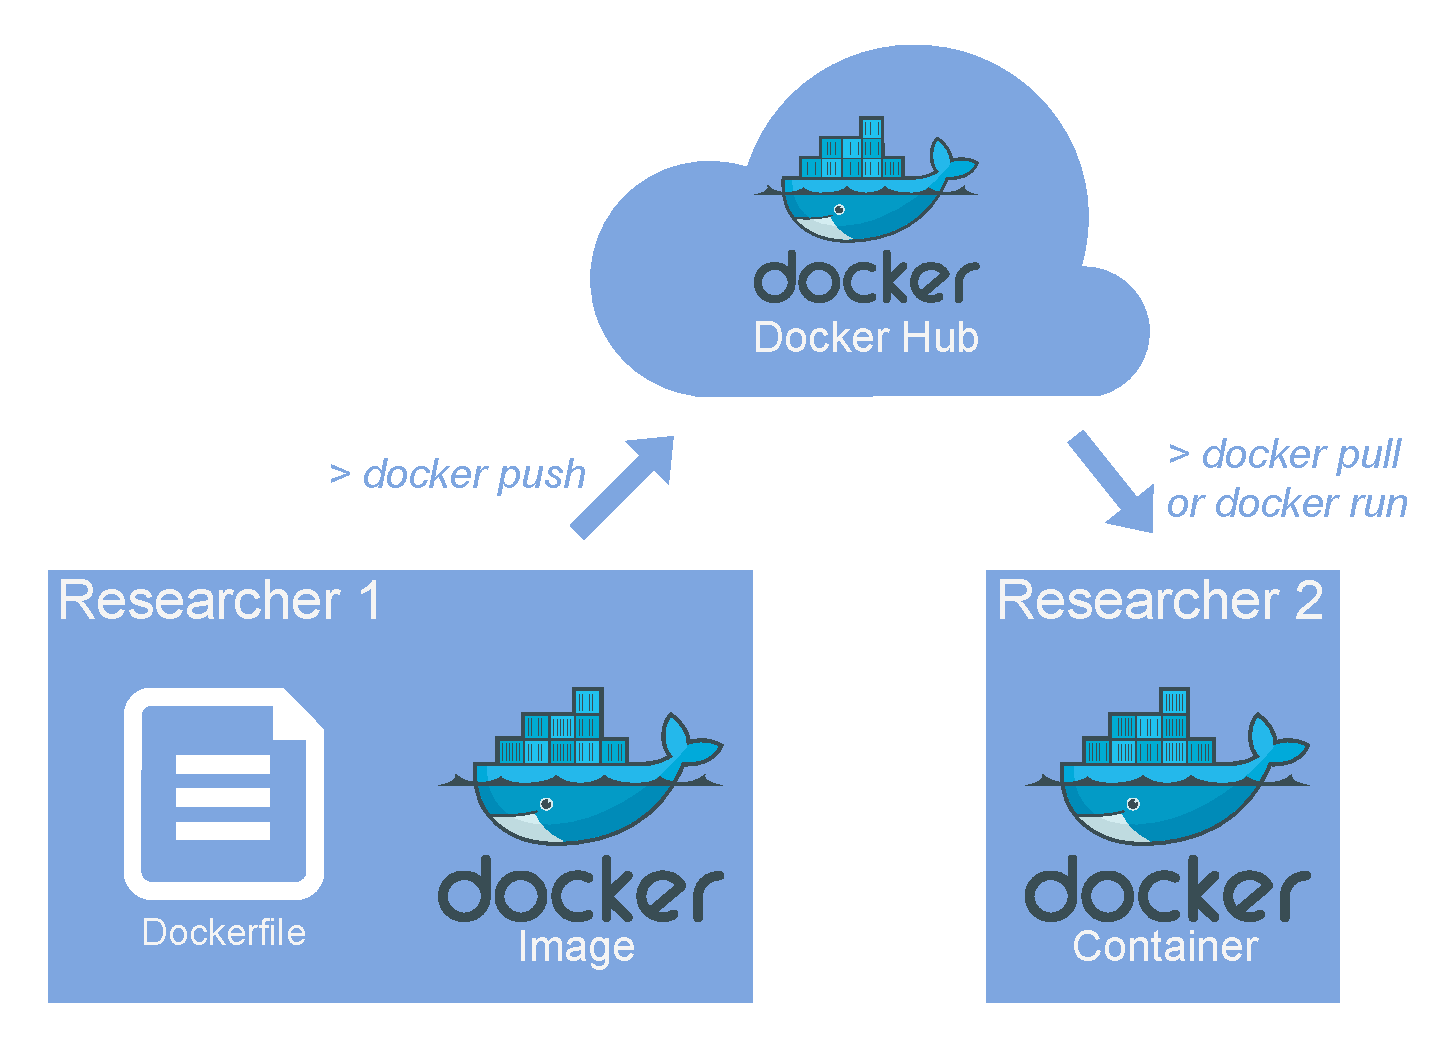
\includegraphics[scale=0.46]{images/fig3.pdf}
  \caption{\textit{Docker} Hub ecosystem and packaging of compiled containers.}
  \label{fig:docker_ecosystem}
\end{figure}

Apart from Docker, there are also compelling language-specific containerisation solutions. These are out the scope of this work because they have not been designed to handle general workflows involving diverse software components, such as the SIOSE-INNOVA project requires. However, even if these solutions were not going to be used, it is interesting to know that in different domains we can find specific solutions for these purposes. As in more general environments, an \textit{R} environment can be reproduced if the correct versions of the interpreter and all packages, libraries, or extension modules are joined together. These dependencies quickly become complicated (the so-called \textit{dependency hell}) so manual documentation is not feasible \cite{nust2017opening}. Several solutions have also emerged to solve these problems in the \textit{R} language \cite{nust2017opening}. Some examples of them are \textit{Packrat}, Renv or \emph{containerit}. \textit{Packrat} is an \textit{R} extension \cite{packrat} which facilitates the process of managing project dependencies. \textit{Renv} \cite{renv} is an \textit{R} package for managing reproducible environments that provides isolation, portability and pinned versions of packages. Finally, \emph{containerit} \cite{nust2019containerit} automates the generation of \textit{Dockerfiles} for \textit{R} workflows, based on images from the Rocker project \cite{boettiger2017introduction}. 

The last practice included in our spectrum is literate programming \cite{knuth1984literate}. This is not used regularly in the SIOSE-INNOVA project, where we focus more on conducting experiments with databases, but it can be useful for compiling always up-to-date versions of most documents derived from the project. One viral initiative used in the \textit{Python} language is \textit{Jupyter} notebooks \cite{kluyver2016jupyter}. \textit{Jupyter} combines comprehensive workflows with narrative text and visualisation of results in a transparent, collaborative, reproducible and reusable way. Similarly, in the \textit{R} field, there are notebooks \cite{hillebrand2015mastering} to combine executable code, rendered visualisations and descriptive text into a single interactive, portable document. Another initiative is the interactive guidelines presented in \cite{trillesSubmitted}, which aim to bring data and code together in a single web document (\textit{Javascript} or \textit{p5.js} \cite{p5js}) and to perform the executions online. 

In order to meet the requirements of SIOSE-INNOVA, we decided to use \textit{Docker} containers to link data and code in a ready to use execution environment. The reason for this selection is due to the broad and general support, adding the possibility to package any piece of software and the workflows between them. As best practices in containerisation, it is necessary to define and share what kind of configuration, connections, dependencies and other details are present in the published containers.

%----------------------------------------------------------

\section{A brief look at the adoption of containerisation in GISc projects}
\label{sec:dockerhub}

Before incorporating docker containers into the project, it was interesting to know how containers are being used in combination with some geospatial technologies. We were specially interested in how to containerise \textit{PostgreSQL/PostGIS} for storing SIOSE data, database clients for performing queries and other tools for processing spatial data. A larger user community would provide a greater number of examples and more available resources. For example, a greater number of geospatial docker images ready to be used or extended. In order to evaluate the level of adoption of these technologies, we performed a systematic review to assess the presence of OSGeo software in the \textit{Docker Hub registry} -- the main repository of docker images.

OSGeo is a community of researchers focused on geospatial software development. Since its inception in 2006, OSGeo has been providing organisational support to build an active international community to advance geospatial technologies and solutions using Free and open-source software (FOSS), open data and open standards. Under the umbrella of OSGeo, we can find a significant number of free and open-source tools in the field of geoinformatics. From the perspective of reproducibility, OSGeo guarantees free access to software (code). OSGeo projects are published under open licences that grant freedom for their use, adaptation and the redistribution of possible modifications. Besides, software included in OSGeo can be installed and used without restrictions in any environment -- commercial or non-commercial -- without any associated cost.

Grouping by software categories, OSGeo promotes desktop GIS applications, libraries for handling map projections, geospatial data conversion tools, geodatabases, geostatistics libraries or web mapping tools, among others. In the OSGeo website, this software is classified into seven different categories, which are: 1) \textit{content management systems}, 2) \textit{desktop applications}, 3) \textit{geospatial libraries}, 4) \textit{metadata catalogues}, 5) \textit{spatial databases}, and 6) \textit{web services}.

In order to perform the systematic review, we extracted the download statistics of \textit{Docker} images (\textit{pulls}) that included OSGeo tools in the \textit{Docker Hub registry}. This review has been carried out by querying the \textit{Docker Registry HTTP API v2} (\url{https://docs.docker.com/registry/spec/api/}).

The semiautomatic search consisted of a series of queries by image name. Thus, we only took into account images containing the name of any of a few selected OSGeo tools. This selection was made depending on whether the tool appeared as featured on the OSGeo website. Query results were sorted by the number of downloads (\textit{pulls}) and limited to a maximum of 1,000 results per search. A \textit{Powershell} script and a \textit{Docker} image to reproduce these queries are available in \url{https://github.com/sergitrilles/OSGEO\_docker} and \url{https://hub.docker.com/repository/docker/strilles/osgeo\_docker} respectively. After running the queries, we revised each returned row to be sure that it was an OSGeo tool. Finally, the results were grouped using the previously mentioned OSGeo software categories, and the total number of downloads by each tool was obtained. This process is described in detail below:

\begin{enumerate}
\item \textit{Selection of OSGeo tools}. There are currently sixty-three different projects indexed on the OSGeo website, including OSGeo projects and community projects. Following the naming convention used on this website in determining featured tools that appears in the main menu, twenty-one tools have been selected from the seven categories defined in Table \ref{tab:tab1}.

\begin{table*}[!ht]
    \begin{center}
        \begin{tabularx}{\textwidth}{l X}
            \hline
            \hline
            \textbf{Category}  & \textbf{Tools} \\ 
            \hline
            \textit{Content Management Systems} & \textit{GeoNode}\\
            \textit{Desktop Applications} & \textit{Marble}, \textit{gvSIG Desktop}, \textit{QGIS Desktop} and \textit{GRASS GIS}\\ 
            \textit{Geospatial Libraries} & \textit{GeoTools}, \textit{Orfeo ToolBox}, \textit{GDAL/OGR} and \textit{GEOS}\\
            \textit{Metadata Catalogues} & \textit{GeoNetwork} and \textit{pycsw}\\
            \textit{Spatial Databases} & \textit{PostGIS}\\
            \textit{Web Mapping} & \textit{MapServer}, \textit{MapFish}, \textit{Deegree}, \textit{OpenLayers}, \textit{GeoMoose}, \textit{Mapbender}, \textit{PyWPS} and \textit{GeoServer}\\ 
            \hline
            \hline 
        \end{tabularx}
    \end{center}
    \caption{List of the selected OSGeo tools considered in our review.}
    \label{tab:tab1}
\end{table*}

\item \textit{Definition of searches}. Searches were defined using the names of the OSGeo tools as query terms. Each search returned the list of images stored in \textit{Docker Hub}, ordered by descending number of downloads (pulls). A filter was applied to set a maximum of 1,000 results in order to ignore residual \textit{Docker} images and build the analysis on those that are widely used.
\item \textit{Execution of searches}. Searches were executed by using the above-mentioned \textit{Docker Registry API}. More specifically, we used a \textit{PowerShell} module called \textit{PSDockerHub} (\url{https://github.com/beatcracker/PSDockerHub}). The results were saved in a \textit{CSV} file for each OSGeo project. From all the images, we obtained the name, description and number of downloads (pulls). 
\item \textit{Manual selection of results}. After the search step, a manual phase is performed to detect possible \textit{Docker} images not related to OSGeo tools. To reach this goal, the returned image results have been verified using the description field to check whether an OSGeo tool is used.
\item \textit{Aggregation and final results}. In the last step, an aggregation is performed on each tool to obtain a total number of downloads.
\end{enumerate}

\begin{table*}[!h]
    \begin{center}
        \begin{tabular}{l l r}
            \hline
            \hline
            \textbf{Category} & \textbf{Tool} & \textbf{Downloads}\\ 
            \hline
            \textit{Content Management Systems} & \textit{GeoNode} & 873,869\\
            \hline
            \textit{Desktop Applications} & \textit{GRASS GIS} & 317\\ 
            & \textit{gvSIG} & 0\\
            & \textit{Marble} & 0\\
            & \textit{QGIS} & 392,882\\
            \hline
            \textit{Geospatial Libraries} & \textit{GDAL/OGR} & 1,653,481\\
            & \textit{GEOS} & 101,165\\ 
            & \textit{GeoTools} & 2,437\\ 
            & \textit{Orfeo Toolbox} & 1,736\\ 
            \hline
            \textit{Metadata Catalogues} & \textit{GeoNetwork} & 2,983,271\\ 
            & \textit{pycsw} & 482,912\\ 
            \hline
            \textit{Spatial Databases} & \textit{PostGIS} & 35,267,083\\ 
            \hline
            \textit{Web Mapping} & \textit{geomoose} & 0\\ 
            & \textit{Degree} & 67\\
            & \textit{Geoserver} & 1,731,538 \\
            & \textit{MapBender} & 986\\ 
            & \textit{MapFish} & 0\\
            & \textit{MapServer} & 1,170,538\\
            & \textit{OpenLayers} & 320,234\\
            & \textit{pywps} & 1,162\\
            \hline
            \hline 
        \end{tabular}
    \end{center}
    \caption{Number of downloads for each OSGeo tool in \textit{Docker Hub}. All results are published in \textit{Zenodo} \cite{Trilles2019}.}
    \label{tab:tab2}
\end{table*}

The results obtained show that the OSGeo category with the highest number of downloads is \textit{spatial databases}, and \textit{PostGIS} is the most \textit{pulled} software with 35,267,083 pulls. The next software with the highest number of downloads is \textit{GeoNetwork} with 2,983,271 within the category of metadata catalogues, followed by \textit{GeoServer} (\textit{web mapping}) and \textit{GDAL/OGR} (\textit{spatial libraries}) with 1,731,538 and 1,653,481, respectively. The \textit{desktop applications} category has the lowest number of downloads among its software options, which is quite normal because \textit{Docker} containers are not initially intended for this purpose. These results show that \textit{PostGIS} is a widely used spatial DBMS in different contexts, while other projects of interest for the SIOSE-INNOVA project have a lower but also important level of adoption (e.g. \textit{GDAL}, \textit{QGIS}).

%----------------------------------------------------------

\section{Enabling research reproducibility in the SIOSE-INNOVA project}
\label{sec:projects}

As a response to the ideas argued in this paper, the SIOSE-INNOVA project made use of several open tools and platforms that were previously mentioned in this manuscript and in the GISc reproducibility spectrum proposed in Figure \ref{fig:GisReproSpectrum}. In sum, different versions and configurations of \textit{PostgreSQL} and \textit{PostGIS} were used for database management, \textit{Geopackages} and \textit{GeoJSON} were our preferred interchange geospatial formats, \textit{GitHub} was used as collaborative development platform and GNU Make was used to compile different database extensions and deliverables (see Section \ref{sec:GISreproducibility}). Finally, containerisation tools (\textit{Docker} and \textit{Docker Compose}) have been used to deploy different workflows, from the simplest to relatively complex ones. In all cases, the necessary tasks have been automated and a second researcher has been able to reproduce the results on a different computer. 

In the following subsections, we explain two different cases where using \textit{Docker} containers made a difference, and we propose the adoption of Unified Modeling Language (UML) diagrams for documenting and visually explaining how \textit{Docker} helped in making some computational experiences more reproducible. These two experiences were developed on a personal computer running Linux \textit{Ubuntu 18.04.3 LTS} (Linux 4.15.0-66-generic) with \textit{Docker} (17.05.0-ce, build 89658be), \textit{docker-compose} (1.11.2, build dfed245), \textit{GNU Make} (v.4.1) and \textit{Bash} (4.4.20(1)-release (x86\_64-pc-linux-gnu)). All the produced code repositories can be found in the project's \textit{GitHub} profile (\url{https://github.com/siose-innova}) and a few container images were stored in \textit{Docker Hub} (\url{https://hub.docker.com/orgs/sioseinnova/repositories}).


\subsection{Benchmarking SQL and NoSQL database models}
\label{subsec:sql_nosql_workflow}

A sophisticated computational experience using SIOSE data was described in detail in \cite{NavarroCarrion2016}. In this case, developed in 2016, an experiment was carried out in which it was verified that specific queries to the SIOSE database could be expedited if the data were stored in a document-oriented database (document store). The experiment consisted in downloading the SIOSE-2005 regional databases, joining them in a single instance, cleaning and renaming tables and columns, duplicating and converting the data to \textit{JSON} format (\textit{JSONB}) and running a battery of thousands of queries on two databases (one relational and the other document-oriented). Despite the complexity of this workflow, a user with minimal instructions would be able to reproduce the experiment (see Figure \ref{fig:sql_nosql_workflow}).

\begin{figure}[!ht]
    \centering
    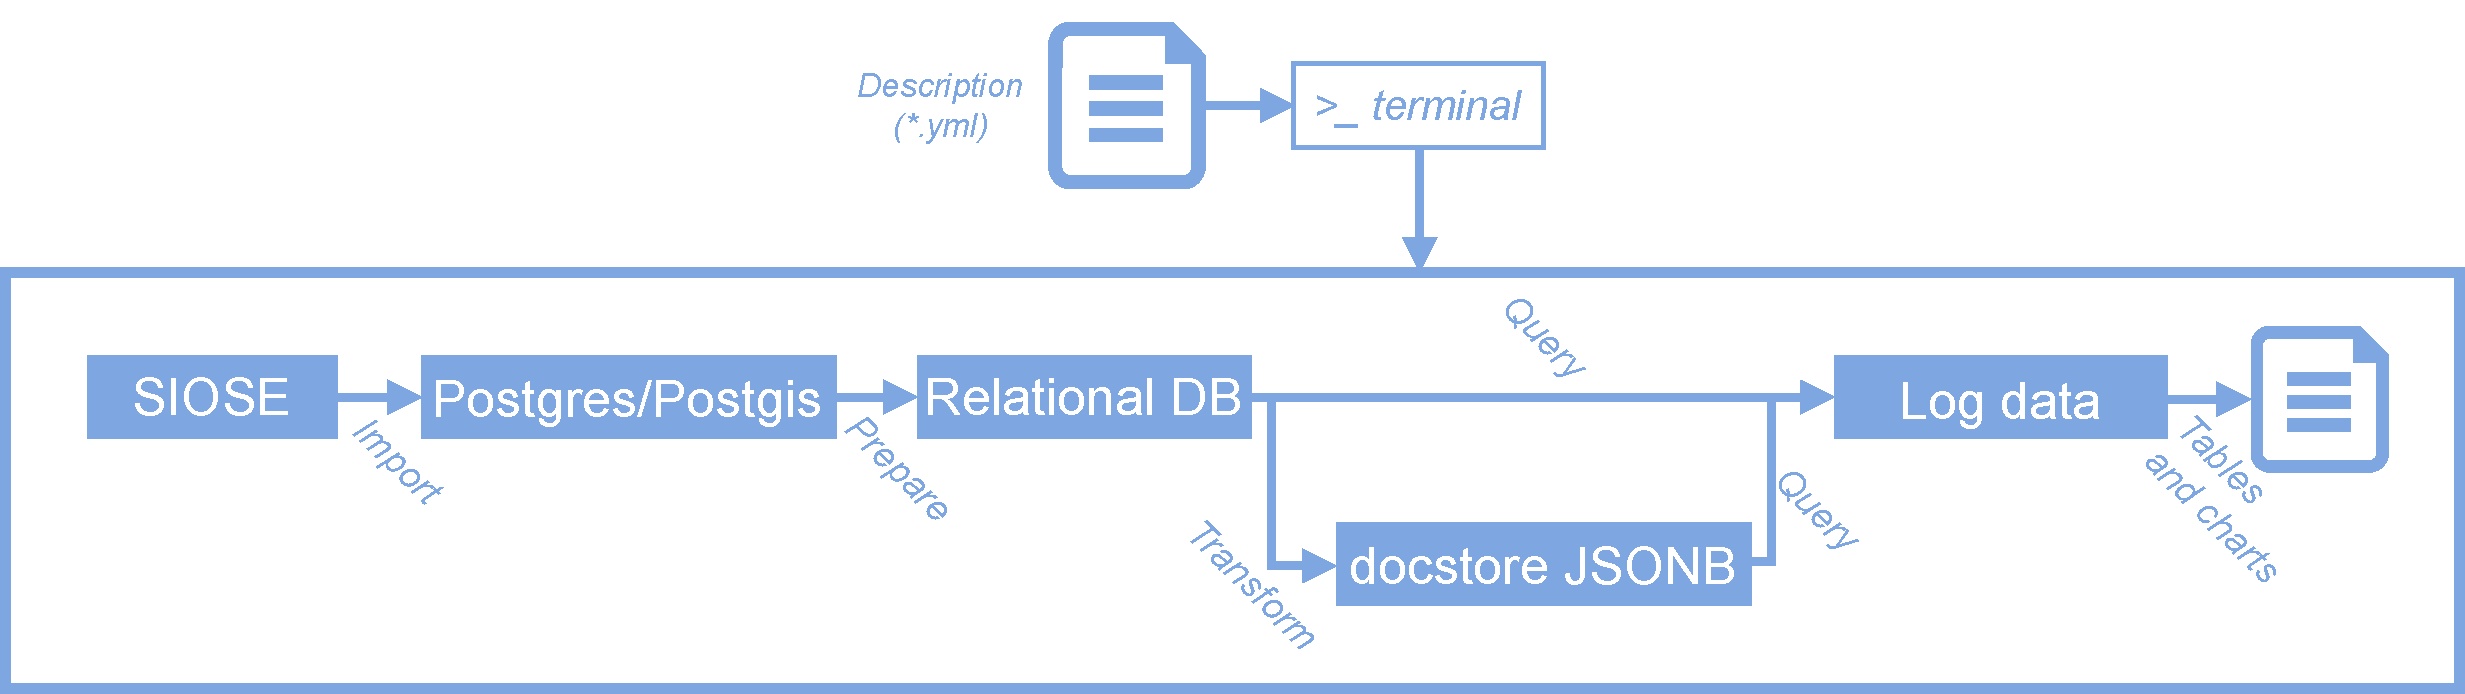
\includegraphics[scale=0.36]{images/fig5.pdf}
    \caption{Computational experience in the SIOSE-INNOVA project \cite{NavarroCarrion2016}.}
    \label{fig:sql_nosql_workflow}
\end{figure}

It should be mentioned that since the experiment was published, we have been able to reproduce it several times without finding any drawbacks related to the reproducibility issues mentioned above (\textit{dependency hell}). In this way, it can be considered that this research is reproducible, according to the concepts proposed in the previous sections (see Figure \ref{fig:GisReproSpectrum}).

The base \textit{Docker} image used in this experiment was built in a personal computer, and then it was uploaded to the \textit{Docker Hub registry} (\url{https://hub.docker.com/repository/docker/labgeo/siose\_2005}). This image can be used as a base image for developing any computational experience over the SIOSE database in a \textit{PostgreSQL/PostGIS} environment. The complete image --containing code, data and environment configuration-- weights 10.5GB, which may not seem very impressive but, when trying to reproduce the experiment, this intermediate step can save up to 5 hours of computing time on a personal computer. This was the time required for downloading and building the SIOSE database from \textit{ESRI personal Geodatabase} files and load that data into a \textit{PostgreSQL}/\textit{PostGIS} database. This image is the base for a \textit{Docker Hub} automated build. All these resources are available in the same repository, together with all the scripts of this experiment (see Figure \ref{fig:sql_nosql_workflow}) \cite{benito_m_zaragozi_2020_3631365}.


\subsection{An ETL process using containerisation}
\label{subsec:siose_splitter}

In this use-case, we used \textit{Docker} containers and other elements presented in Section \ref{sec:GISreproducibility} to prepare a reproducible ETL workflow (Extract-Transform-Load). In order to split the SIOSE database into small portable GIS files, we wrote all the necessary scripts (\textit{Bash}, \textit{Makefile} or spatial-\textit{SQL}) and designed them to deploy all the necessary tools \cite{benito_m_zaragozi_2020_3631365}. This workflow is shown in more detail in the UML activity diagram in Figure \ref{fig:siose_splitter_workflow}. The proposed diagram separates those tasks that need to be performed by the researcher and those that were completely automated. The steps can be deployed by using a Makefile and are enumerated as follows:

\begin{enumerate}
    \item The user launches the workflow using several \textit{docker run} commands or one single execution of the deployment software (\textit{docker-compose up}).
    \item \textit{Docker} starts all the necessary services sequentially (see Figure \ref{fig:siose_splitter_stack}).
    \item A \textit{PostgreSQL/PostGIS} server is started which already contains a preloaded SIOSE database.
    \item \textit{SQL} scripts are executed from the \textit{Makefile}, creating spatial grids and statistics that will be used to split the database into GIS portable files. \textit{GNU Make} will ensure that all files are created, and it will prevent any unnecessary overwrite operations from being carried out on any file. 
    \item Then, the process loops over the cells of several spatial grids at different mapping scales.
    \item In every iteration, a spatial query is executed and intersects the SIOSE database with the corresponding area of interest (cell grid).
    \item Using the \textit{GDAL}/\textit{OGR} library, the selected SIOSE polygons together with a selection of LU/LC attributes are written into a new \textit{Geopackage} file. 
    \item This new \textit{Geopackage} is compressed and stored in the working directory.
    \item Then the user can inspect the database or check the produced outputs using a containerised version of \textit{PGadmin4} or \textit{QGIS}.
    \item When the user stops the process, \textit{Docker} stops all services and frees all the unused computing resources.
\end{enumerate}{}

\begin{figure}[!ht]
    \centering
    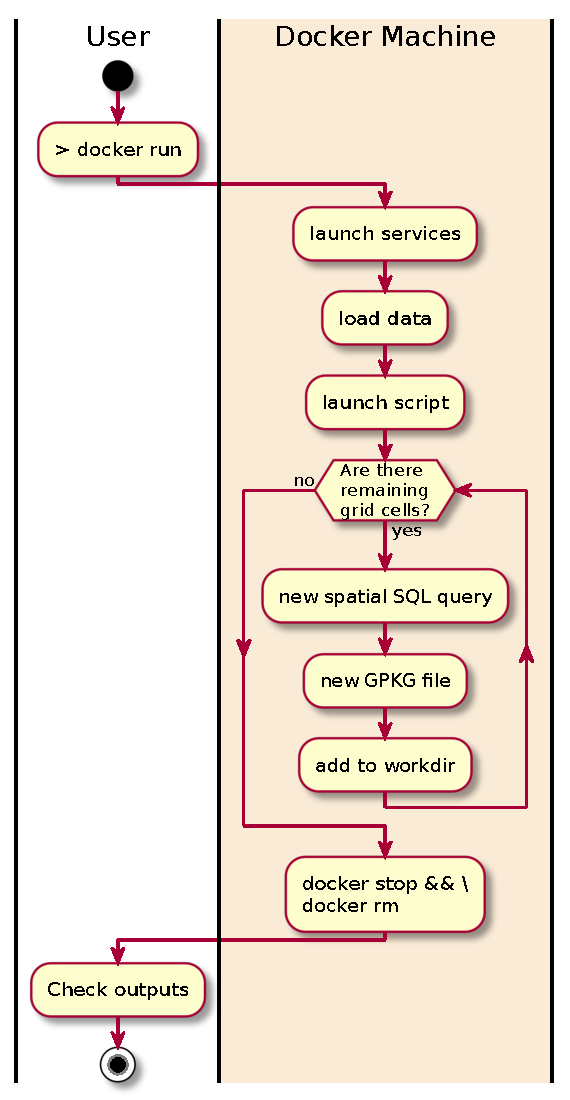
\includegraphics[width=0.5\textwidth]{images/siose-splitter-activity-diagram.pdf}
    \caption{UML activity diagram showing all the tasks automated in the SIOSE-splitter solution.}
    \label{fig:siose_splitter_workflow}
\end{figure}

Launching this workflow should be straightforward for researchers familiar with these technologies. However, when it comes to adapting it for other purposes, the process may become far more complicated (e.g. using other database versions or different output formats, or testing new software configurations, among other possibilities). There are several scripts, software extensions, \textit{Makefiles}, queries and \textit{Dockerfiles} that have been developed specifically for this workflow. Besides, due to the \textit{Docker} inheritance mechanisms mentioned in Section \ref{sec:containerization}, many configuration options or resources could be hidden in the development process. That being said, this workflow is more complicated at this level of detail. For this reason, we propose using UML diagrams to document such complex deployments.

The UML components diagram in Figure \ref{fig:siose_splitter_stack} shows the static part of the deployment required for this workflow to be run. The correct use of these diagrams for documentation can facilitate the understanding of essential parts of the working environment without the need to revise all the dependencies systematically. In this diagram, we show what happens inside and outside the \textit{Docker} environment. As an example of hidden configurations, in this diagram, we are showing ports and software dependencies. This aspect is essential because these details are not available in our \textit{Dockerfiles}, since they are in other base images from which they inherit. One example of these details is the port 5433 added to map a \textit{PostgreSQL} server in Figure \ref{fig:siose_splitter_stack}. This application usually uses 5432 as a default TCP port. However, using this port in a container could become in conflict with a \textit{PostgreSQL} server running on the host machine. In this case, the diagram (Figure \ref{fig:siose_splitter_stack}) shows that the container port is mapped to avoid such type of problem.

According to the diagram of the components, the user has many possibilities to inspect the workflow and its outputs without knowing anything about the operating systems and configurations running under the surface: 1) use the system console to execute new \textit{Docker} commands; 2) check the produced geopackages transparently in a folder mounted in the host machine; 3) connect a \textit{Postgres} client using port 5433; 4) make use of a \textit{PgAdmin4} web client running on port 5050; and 5) use a dockerised version of \textit{QGIS} both for exploring new GIS files or for connecting to the SIOSE database running in the \textit{Docker} container. As can be seen from the number of \textit{QGIS} pulls in \textit{Docker Hub} (see Table \ref{tab:tab2}), using a containerised version of \textit{QGIS} is a practice that may have some interest. Besides, it is interesting to mention that, as can be seen from the component diagram, it would be easy to launch more than one instance of \textit{QGIS} in its different versions. This approach can be interesting both in development tasks and in more routine tasks in which having a specific \textit{QGIS} version may be necessary. The \textit{QGIS} API documentation can be useful for checking major changes that could affect reproducibility (\url{https://qgis.org/api/api_break.html}).

\begin{figure}[!ht]
    \centering
    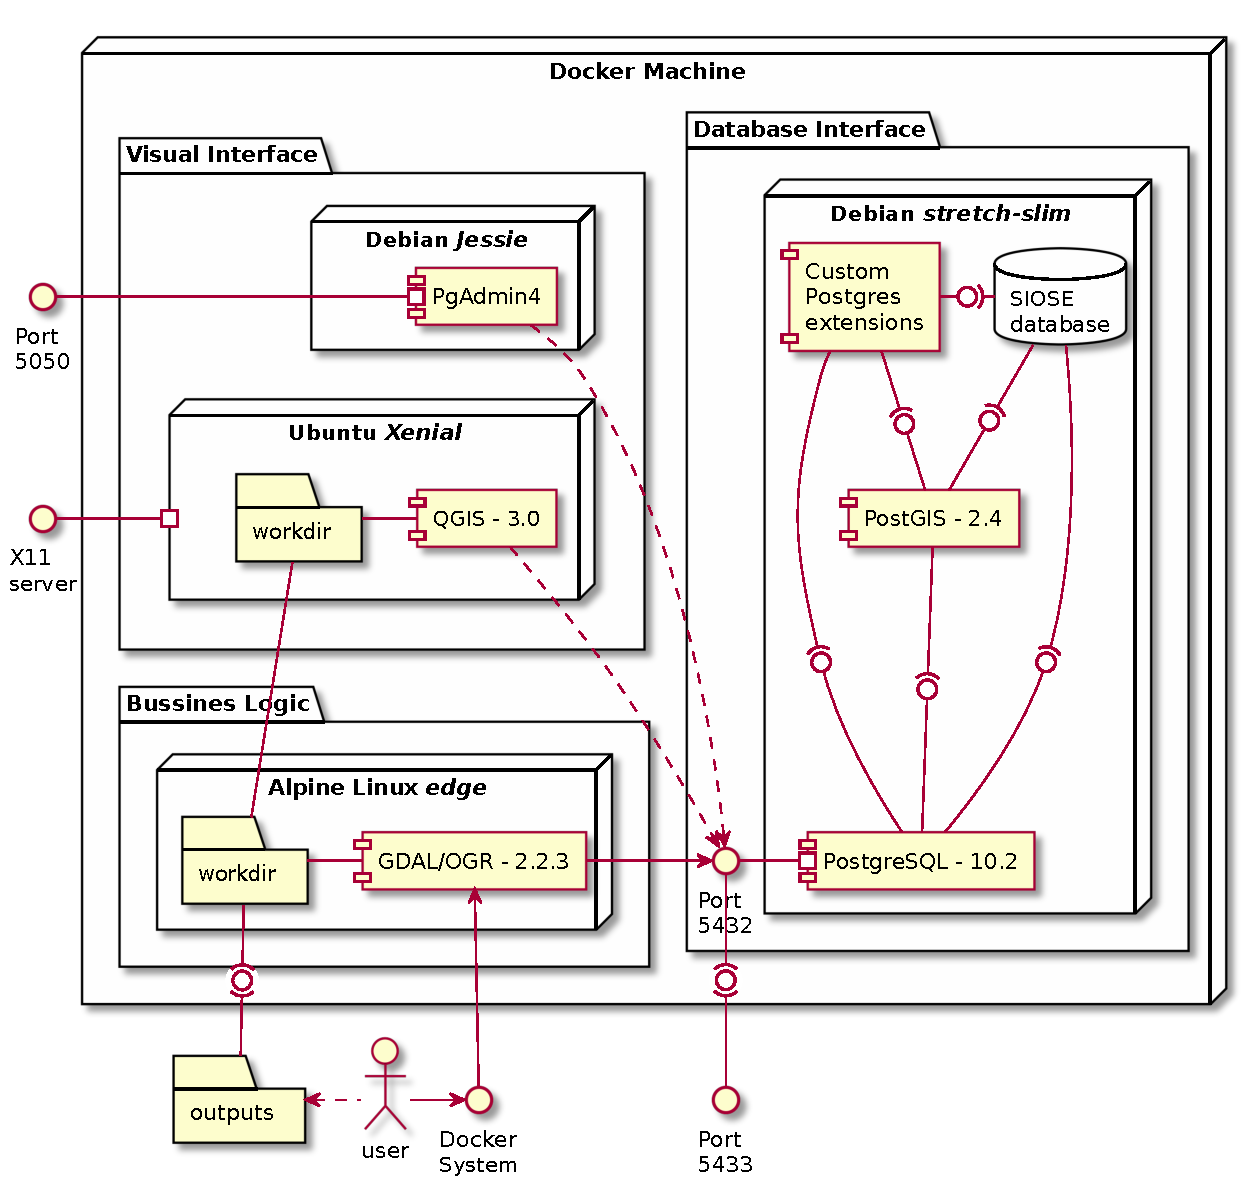
\includegraphics[width=.9\textwidth]{images/siose-splitter-deployment-diagram.pdf}
    \caption{UML components diagram showing the containers and configurations used in the SIOSE-splitter solution.}
    \label{fig:siose_splitter_stack}
\end{figure}


%----------------------------------------------------------

\section{Concluding remarks}
\label{sec:conclusions}

The challenges of reproducible science are systemic and generally costly to address. However, there is a consensus among researchers on the need to improve collaborative work and scientific rigour to overcome these obstacles. The latest experiences in different fields recommend the use of open data, open software and reproducible workflows. In recent years, many new resources have become popular and have reached a sufficient level of maturity to be applied in GISc projects.

Once the need for higher reproducibility in research is accepted, more and more researchers are encouraged to incorporate new tools and good practices into their projects. In this paper, we have described the necessary decision-making to make the SIOSE-INNOVA project more reproducible, selecting OSGeo tools, choosing standards-based files and trying to explain our research in the best possible way. This includes open-source code and data with a good description of workflows, among other desirable features. This concern for reproducibility began internally within the project -- all researchers in the SIOSE-INNOVA project should be able to reproduce the work of other colleagues -- but it has led to features that can be beneficial even after the project ends.

In the process, we have learned that there are currently many resources that can be used to increase the reproducibility of a GIScience investigation. Therefore, it is essential to know the different options available and know what they contribute to the research. Given the complexity of this scenario, we have tried to organise these elements in a diagram based on the spectrum of reproducibility proposed by Peng \cite{peng2011reproducible}. This schema has been described throughout Section \ref{sec:GISreproducibility}. The relationships between tools and practices of such a diverse nature are complex to be described in a single diagram, so there is still room for improvement to develop a more comprehensive and precise representation, maybe a GIScience ORR map. However, even with all the qualifications that can be made, our spectrum of reproducibility in GISc has allowed us to realise that, to a greater or lesser extent, it is possible to improve the reproducibility of some computational experiences without significantly deviating from the original objectives of the project. Even before considering reproducibility as a cross-cutting objective of the SIOSE-INNOVA project, some techniques, standards and practices that favour reproducibility were already being applied. For example, the use of FOSS GIS for economic reasons, the publication of SIOSE data with an open license due to legal constraints, the distribution of data in standard and well-known formats or the need for collaborative work among members of the same research team. All these issues also have their advantages in terms of reproducibility of research. Other elements were new to the project researchers or involved an additional effort to be used in some computational experiences. The most prominent case has been the use of \textit{Dockers} to package workflows of a certain level of complexity and be able to distribute them to the other members of the project (or external researchers).

Before applying Dockers to our project and to better understand the level of adoption of containerisation technologies in GIScience, we carried out a systematic review of the official \textit{Docker registry} \textit{(Docker Hub}). In section \ref{sec:dockerhub}, we measured the presence of the most popular geospatial solutions supported by the OSGeo community in \textit{Docker Hub}. Our results show that the most frequently attended software category is spatial databases using \textit{PostGIS} software, followed by the metadata catalogue category, where \textit{GeoNetwork} is the most recurrent option. Other containerised tools like \textit{QGIS} were of interest in achieving our objectives. The level of adoption of these resources -- containerised OSGeo projects -- is considerable, which means that there are many examples and use cases available, making it easier to start using them. Of course, this is a shallow review that should be better addressed in the near future. There are many questions to answer about the level of adoption of containers in GISc (e.g. user census and profiles, pull trends, the purpose of the images stored in \textit{Docker Hub}, diversity of environments, among other interesting topics).

Once we defined our working environment for the SIOSE-INNOVA project, we performed some computational experiences that are described in Section \ref{sec:projects}. During these experiences, we used different technology stacks to achieve a high level of reproducibility (e.g. version control, open geospatial libraries, containerisation platforms). The tools used and the proposed workflows make up one solution among many other possibilities. As mentioned above, one of the main problems that may arise is that the tools mentioned and other aspects of reproducible research are not part of the processes currently used by researchers. Although simple in general, these tools entail additional training for everyone involved and imply coordinated tasks that can eventually become more complex. This extra burden for researchers is not directly rewarded and, as noted, the pressure to publish research may be so high that there is no room to try to introduce these improvements \cite{Baker2016}. However, attempting to conduct reproducible research, as shown in the GISc reproducibility spectrum, is not only related to sophisticated technologies, but also to paying attention to certain decisions, such as choosing an appropriate code and data licence, or trying to make the necessary effort in documenting the research. For example, some first steps could be to write \textit{README} files or to create concise diagrams to explain the purpose of the research in a better way. As a minor contribution of this work, we propose how to describe a dockerised workflow using UML diagrams.

Derived from our previous considerations, it must be emphasised that, in this work, only the technological approach has been evaluated for the problem of low scientific reproducibility. However, the issue as a whole needs to be addressed more comprehensively, as solutions depend on a change in the attitude of the scientific community. As can be seen from our GISc spectrum of reproducibility, there are many tools and mechanisms to promote research reproducibility -- regardless of whether they are specific to the geospatial domain or inherited from other disciplines -- and so trying to conduct reproducible research or achieving is highly related to the level of commitment \cite{nust2018reproducible}. For future work, we intend to keep applying best practices required to achieve a better level of reproducible research. 


%%%%%%%%%%%%%%%%%%%%%%%%%%%%%%%%%%%%%%%%%%
\vspace{6pt} 

%%%%%%%%%%%%%%%%%%%%%%%%%%%%%%%%%%%%%%%%%%
%% optional
%\supplementary{The following are available online at \linksupplementary{s1}, Figure S1: title, Table S1: title, Video S1: title.}

%%%%%%%%%%%%%%%%%%%%%%%%%%%%%%%%%%%%%%%%%%
\authorcontributions{Conceptualisation, Sergio Trilles and Benito Zaragozí; Formal analysis, Sergio Trilles; Funding acquisition, Sergio Trilles; Methodology, Benito Zaragozí; Software, José Tomás Navarro-Carrión and Benito Zaragozí; Supervision, Benito Zaragozí; Writing – original draft, Sergio Trilles and Benito Zaragozí; Writing – review \& editing, José Tomás Navarro-Carrión.}

%%%%%%%%%%%%%%%%%%%%%%%%%%%%%%%%%%%%%%%%%%
\funding{This work has been funded by the Generalitat Valenciana through the ``Subvenciones para la realización de proyectos de I+D+i desarrollados por grupos de investigación emergentes'' programme (GV/2019/016) and by the Spanish Ministry of Economy and Competitiveness under the subprogrammes Challenges‐Collaboration 2014 (RTC‐2014‐1863‐8) and Challenges R+D+I 2016 (CSO2016‐79420-R AEI/FEDER, EU). Sergio Trilles has been funded by the postdoctoral programme PINV2018 - Universitat Jaume I (POSDOC-B/2018/12) and stays programme PINV2018 - Universitat Jaume I (E/2019/031).}

%\funding{The authors appreciate the support provided by the Ministry of Economy and Competitiveness under the subprograms Challenges ‐ Collaboration 2014 (RTC ‐ 2014‐1863‐8) and Challenges R + D + I 2016 (CSO2016‐79420 ‐ R AEI / FEDER, EU).}

%%%%%%%%%%%%%%%%%%%%%%%%%%%%%%%%%%%%%%%%%%
%\acknowledgments{In addition, we also want to thank the collaboration provided by the Land Occupation Service of the National Geographic Institute (IGN).}

%%%%%%%%%%%%%%%%%%%%%%%%%%%%%%%%%%%%%%%%%%
% Citations and References in Supplementary files are permitted provided that they also appear in the reference list here. 

%=====================================
% References, variant A: internal bibliography
%=====================================
\bibliography{bibliography.bib}

% The following MDPI journals use author-date citation: Arts, Econometrics, Economies, Genealogy, Humanities, IJFS, JRFM, Laws, Religions, Risks, Social Sciences. For those journals, please follow the formatting guidelines on http://www.mdpi.com/authors/references
% To cite two works by the same author: \citeauthor{ref-journal-1a} (\citeyear{ref-journal-1a}, \citeyear{ref-journal-1b}). This produces: Whittaker (1967, 1975)
% To cite two works by the same author with specific pages: \citeauthor{ref-journal-3a} (\citeyear{ref-journal-3a}, p. 328; \citeyear{ref-journal-3b}, p.475). This produces: Wong (1999, p. 328; 2000, p. 475)

%=====================================
% References, variant B: external bibliography
%=====================================
%\externalbibliography{yes}
%\bibliography{your_external_BibTeX_file}
%%%%%%%%%%%%%%%%%%%%%%%%%%%%%%%%%%%%%%%%%%
%% optional
%\sampleavailability{Samples of the compounds ...... are available from the authors.}
%%%%%%%%%%%%%%%%%%%%%%%%%%%%%%%%%%%%%%%%%%
\end{document}

